% Zakladne parametre a jazyk dokumentu
\documentclass[12pt,twoside]{report}
\usepackage[utf8]{inputenc}
\usepackage[slovak]{babel}

% Aby som mohol davat priamu rec
\usepackage{dirtytalk}

% Obrazky
\usepackage{graphicx}
\graphicspath{ {images/} }

% Uloz obrazok tam, kde je deklarovany - nie tam, kde si latex zmysli (na vrch stranky, na novu stranku a tak)
\usepackage[section]{placeins}

% Cislovanie obrazkov a tabuliek
\usepackage{chngcntr}
%Cisluj obrazky nezavisle od cisla kapitol/podkapitol
\counterwithout{figure}{chapter}
\counterwithout{table}{chapter}

% Formatovanie strany
\usepackage{caption}
\usepackage{subcaption}
\usepackage[a4paper,width=150mm,top=25mm,bottom=25mm,bindingoffset=6mm]{geometry}

% Hlavicka a pata

\usepackage{fancyhdr}
\pagestyle{fancy}
\fancyhead{}
%\fancyhead[RO,LE]{Implementácia firemnej siete}
%\fancyfoot{}
%\fancyfoot[LE,RO]{\thepage}
%\fancyfoot[LO,CE]{Kapitola \thechapter}
%\fancyfoot[CO,RE]{Author Name}
%\renewcommand{\headrulewidth}{0.4pt}
%\renewcommand{\footrulewidth}{0.4pt}

% Bibliografia
\usepackage[style=authoryear,sorting=none]{biblatex}
\addbibresource{references.bib}

% Metadata
\title{Implementácia firemnej siete}
\author{Andrej Hucík, Miroslav Kozák, Andrej Šišila}
\date{26.2. 2017}

\begin{document}

\begin{titlepage}
    \begin{center}
        \vspace*{1cm}
        
        \Huge
        \textbf{Thesis Title}
        
        \vspace{0.5cm}
        \LARGE
        Thesis Subtitle
        
        \vspace{1.5cm}
        
        \textbf{Author Name}
        
        \vfill
        
        A thesis presented for the degree of\\
        Doctor of Philosophy
        
        \vspace{0.8cm}
        
        
\includegraphics[width=0.4\textwidth]{university}
        
        \Large
        Department Name\\
        University Name\\
        Country\\
        Date
        
    \end{center}
\end{titlepage}


% abstrakt vypustime
%\thispagestyle{plain}
\begin{center}
    \Large
    \textbf{Thesis Title}
    
    \vspace{0.4cm}
    \large
    Thesis Subtitle
    
    \vspace{0.4cm}
    \textbf{Author Name}
    
    \vspace{0.9cm}
    \textbf{Abstract}
\end{center}
Lorem ipsum dolor sit amet, consectetur adipisicing elit, sed do eiusmod tempor incididunt ut labore et dolore magna aliqua. Ut enim ad minim veniam, quis nostrud exercitation ullamco laboris nisi ut aliquip ex ea commodo consequat. Duis aute irure dolor in reprehenderit in voluptate velit esse cillum dolore eu fugiat nulla pariatur. Excepteur sint occaecat cupidatat non proident, sunt in culpa qui officia deserunt mollit anim id est laborum.

Lorem ipsum dolor sit amet, consectetur adipisicing elit, sed do eiusmod tempor incididunt ut labore et dolore magna aliqua. Ut enim ad minim veniam, quis nostrud exercitation ullamco laboris nisi ut aliquip ex ea commodo consequat. Duis aute irure dolor in reprehenderit in voluptate velit esse cillum dolore eu fugiat nulla pariatur. Excepteur sint occaecat cupidatat non proident, sunt in culpa qui officia deserunt mollit anim id est laborum.

Lorem ipsum dolor sit amet, consectetur adipisicing elit, sed do eiusmod tempor incididunt ut labore et dolore magna aliqua. Ut enim ad minim veniam, quis nostrud exercitation ullamco laboris nisi ut aliquip ex ea commodo consequat. Duis aute irure dolor in reprehenderit in voluptate velit esse cillum dolore eu fugiat nulla pariatur. Excepteur sint occaecat cupidatat non proident, sunt in culpa qui officia deserunt mollit anim id est laborum.


\tableofcontents

\listoffigures

%\listoftables

\chapter{Úvod}
\paragraph{}
Základom každej firmy, či už malej, strednej alebo veľkej, je stabilná a bezpečná sieťová infraštruktúra.
\paragraph{}
V našej práci sa budeme zaoberať implementáciou a konfiguráciou menšej firemnej siete, ktorá bude pozostávať z jedného smerovača, jedného prepínača, dvoch serverových systémov a dvoch pracovných staníc. Potom na potrebných uzloch nastavíme potrebné služby, ktoré umožnia firme poskytovať služby pre vnútornú, ale aj vonkajšiu sieť.


\chapter{Ciele práce}
\paragraph{}
Hlavným cieľom našej práce je vytvorenie jednoduchej sieťovej infraštruktúry, ktorú bude možné nasadiť do podnikového prostredia. Vytvorenie a konfigurácia takejto siete si vyžadovalo splnenie nasledovných čiastkových cieľov:
\begin{itemize}
\item Inštalácia operačného systému na serverové systémy, pracovné stanice a smerovač, a ich následná základná konfigurácia
\item DNS: Master/Slave riešenie s replikáciou a overením
\item Podpora viacerých virtuálnych web serverov a s inštaláciou niektorej z web aplikácii typu CMS or Wiki
\item Firewall na smerovači cez  netfilter s NAT
\item Firewall na server systémoch
\item NTP čas pre firmu
\item SSH prístup
\item DHCP
\item Email
\end{itemize}
\paragraph{}
Služby bolo potrebné sprevádzkovať najprv na linuxovej distribúcií Debian 8.6.0 x64 Stable a potom aj na Windows Server 2016, preto je aj táto práca rozdelená na dve hlavné časti: konfiguráciu v prostredí Windows a Linux.


\chapter{Topológia siete}
\paragraph{}
Naša topológia siete pozostáva z firewallu ku ktorému je na jednom rozhraní pripojený prepínač ku ktorému su napojené dva servery a dva počítače. Na druhom rozhraní je Internet. Na linuxoch aj na windowsoch bola rovnaká topológia s výnimkou, že pri pracovaní s linuxom sa nachádzali počítače a servery v rozdielnych VLAN: Servery vo VLAN-e 10 a desktopy vo VLAN-e 20.
\paragraph{}
Keďže si Windows Server nerozumel s VLAN-ami, topológia siete sa líši v tom, že všetky koncové uzly sú v defaultnej VLAN-e (VLAN 1).



\chapter{Linux}
\section{Inštalácia operačného systému}
\paragraph{}
Ako serverový aj klientský operačný systém sme použili linuxovú distribúciu \say{Debian 8.6.0 x64 - kódové meno \say{Jessie} }Najprv sme si stiahli inštalačný iso súbor s \say{Debian 8.6.0 stable 64 bit} vo verzií \say{netinst} t.j. operačný systém si sťahuje aktuálne balíčky z internetu.
\paragraph{}
V rámci nastavení počítačov (serverov a desktopov) vo VirtualBox-e sme zmenili tieto nastavenia:
\begin{itemize}
\item System -\textgreater{} Motherboard -\textgreater{} Base memory = 1024MB
\item System -\textgreater{} Processor -\textgreater{} Processor(s) = 1 CPU
\item System -\textgreater{} Processor -\textgreater{} Enable PAE/NX = zaškrtnúť
\item System -\textgreater{} Acceleration -\textgreater{} Hardware Virtualization -\textgreater{} Enable VT-x/AMD-V = zaškrtnúť
\item Storage -\textgreater{} Controller: IDE -\textgreater{} klikneme na Empty disk -\textgreater{} v pravom paneli klikneme na ikonku CD a vyberieme možnosť Choose Virtual Optical Disk File. Otvorí sa dialógové okno, v ktorom vyhľadáme stiahnutý iso súbor.
\item Pre servery a desktopy: Network -\textgreater{} Adapter 1 -\textgreater{} Enable Network Adapter a nastavíme Attached to -\textgreater{} Bridged Adapter -\textgreater{} eth1. Sieťové nastavenia pre firewall sú rovnaké, ako pre desktopy a servery, s tým, že Adapter 1 sme nastavili na Bridged Adapter pripojený na eth1 (lokálne rozhranie) a navyše sme zapli aj Adapter 2 ako Bridged Adapter pripojený na eth0 (verejné rozhranie).
\end{itemize}

\paragraph{}
Po nastavení virtuálky sme ju spustili. Ďalej sme postupovali v štandardnej inštalácií Debian-u. Ako doménu sme nastavili takú, ktorá nám bola pridelená: \say{sos3.local}. Ako hostname sme nastavili doménové meno, ktoré je odvodené od jej funkcie napr. všetky servery majú označenie \say{SX} a desktopy \say{DX}, kde X je poradové číslo servera/desktopu. Z doplnkový balíškov sme pre servery neinštalovali nič, jedine pre desktopy sme nainštalovali grafické rozhranie XFCE.

\section{Základná konfigurácia}
\paragraph{}
Každý inštalácia Debian-u obsahovala navyše tieto balíčky (inštalovali sme ich príkazom \say{sudo apt-get install}):\\
tcpdump vim openssh-client openssh-server

\section{VLAN}
\paragraph{}
Servery sú vo VLAN 10, desktopy vo VLAN 20. Smerovanie medzi VLANami je vykonávané na FW. Preto sme na FW museli nainštalovať balíčky \say{isc-dhcp-server} a \say{vlan} t.j. \say{apt-get install isc-dhcp-server vlan}. Potom sme editovali súbor \say{/etc/network/interfaces} tak, že sme odstránili adresné informácie z vnútorného interfacu eth1, ale nechali sme \say{auto eth1}, aby sa port zapol (UP). Následne sme pridali subinterface eth1.10 pre VLAN 10 (servery) a eth1.20 pre VLAN 20 (desktopy). Adresný rozsah pre jednotlivé VLAN bola sieť 192.168.0.0/24 rozdelená na dve /25 siete: 192.168.0.0 - 192.168.0.127 pre VLAN 10 a 192.168.0.128 - 192.168.0.255 pre VLAN 20
\paragraph{}
FW je DHCP Relay server. Všetky DHCP požiadavky prepošle FW DHCP serveru, ktorý pridelí klientovi IP adresu a ďalšie nakonfigurované informácie. Týmto spôsobom je FW zodpovedný iba za filtrovanie premávky a server za služby poskytované na sieti. IP adresa DHCP servera sa do konfiguračného súboru \say{/etc/default/isc-dhcp-relay} DHCP relay agenta musí zadať BEZ úvodzoviek a musíme počúvať na obidvoch podrozhraniach t.j. eth1.10 aj eth1.20. Konfigurácia DHCP Relay servera je uvedená nižšie.

\noindent
{\fontfamily{qcr}\selectfont

% Urob text mensi, aby sa vosiel na sirku obrazovky
\begin{small}

% Pouzijeme "verbatim", aby sme escapeovali cely odsek
\begin{verbatim}

# Defaults for isc-dhcp-relay initscript
# sourced by /etc/init.d/isc-dhcp-relay
# installed at /etc/default/isc-dhcp-relay by the maintainer scripts

#
# This is a POSIX shell fragment
#

# What servers should the DHCP relay forward requests to?
# Forwarduj DHCP poziadavky na S2
SERVERS=192.168.0.3

# On what interfaces should the DHCP relay (dhrelay) serve DHCP requests?
#Pocuvame DHCP REQUESTY na vlane 20 pre desktopy, ale aj na vlane 10, aby sme mohli REQUEST poslat na server
INTERFACES="eth1.10 eth1.20"

# Additional options that are passed to the DHCP relay daemon?
OPTIONS=""

\end{verbatim}

\end{small}

}

\section{DNS}
\paragraph{}
Systém názvov domén alebo systém mien domén, alebo systém doménových mien (Domain Name System), skr. DNS, je systém, ktorý ukladá prístup k informácii o názve stroja (hostname) a názve domény v istej distribuovanej databáze v počítačových sieťach ako internet. Najdôležitejšie je, že poskytuje mechanizmus získania IP adresy pre každé meno stroja (lookup) a naopak (reverse), a uvádza poštové servery (MX záznam) akceptujúce poštu pre danú doménu.
\paragraph{}
DNS poskytuje na internete všeobecne dôležitú službu, pretože kým počítače a sieťový hardvér pracujú s IP adresami, ľudia si vo všeobecnosti ľahšie pamätajú mená strojov a domén pri použití napr. v URL a e-mailovej adrese (obzvlášť nepríjemné by to bolo pri IPv6 adrese). DNS tak tvorí prostredníka medzi potrebami človeka a softvéru.
\paragraph{}
V rámci našej doménovej zóny \say{sos3.local} sme si museli nastaviť dva DNS servery: Master (S1) a Slave (S2). Slave zrkadlí hlavný DNS server a v prípade poruchy ho zastúpi. Keďže si Slave DNS server všetko stiahne z Master DNS servera, netreba ho primárne konfigurovať, ale stačí mu  nastaviť \say{allow-transfer} na privátnu IP Master DNS.
\paragraph{}
Na obidva servery sme nainštalovali DNS server a nástroje na overenie jeho funkčnosti príkazom \say{apt-get install bind9 bind9utils dnsutils}.
\paragraph{}
Master DNS serveru sme upravovali súbory \say{/etc/resolv.conf} (konfigurácia adries DNS serverov), \say{/etc/bind/master/db.sos3.local} (view-lokálny), \say{/etc/bind/master/db.sos3.external} (view-verejný), \say{/etc/bind/named.conf.local} (definovanie lokálnych a verejných DNS View). Obsah súboru \say{/etc/resolv.conf} je uvedený nižšie.

\noindent
{\fontfamily{qcr}\selectfont

% Urob text mensi, aby sa vosiel na sirku obrazovky
\begin{small}

% Pouzijeme "verbatim", aby sme escapeovali cely odsek
\begin{verbatim}

domain sos3.local
nameserver 192.168.0.2
nameserver 192.168.0.3

\end{verbatim}

\end{small}

}

\paragraph{}
V adresári \say{/etc/bind} na S1 sme vytvorili adresár \say{master}, do ktorého sme ukladali zónové súbory pre DNS.
\paragraph{}
Viewy sme nastavovali na Master  DNS serveri súbormi \say{/etc/bind/named.conf.local}, \say{/etc/bind/master/db.sos3.local}, \say{/etc/bind/master/db.sos3.external}. Pri dotazovaní na doménové meno nášho DNS zvnútra sa použijú privátne adersy DNS serverov zo súboru \say{/etc/bind/master/db.sos3.local}. Pri dotazovaní na doménové meno nášho DNS zvonku sa použijú verejné adersy DNS serverov zo súboru \say{/etc/bind/master/db.sos3.external}. O tom, aký súbor sa použije, rozhoduje súbor \say{/etc/bind/named.conf.local}
\paragraph{}
Počítače v lokálnej sieti sa dokážu navzájompingať pomocou svojich hostname. Preklad hostname názvov na IP adresy je definovaný v súbore \say{/etc/bind/master/db.sos3.local}.
\paragraph{}
Firewall bol nakonfigurovaný tak, aby prepúšťal DNS požiadavky na lokálnej sieti, a tiež aby prepúšťal požiadavky z internetu na obidva DNS servery t.j. aby boli obidva DNS servery viditeľné zvonku (PREROUTING). Záznamy pre DNS sú pre obidve verejné IP adresy pre udp aj tcp port 53 (zdrojový aj cieľový).
\paragraph{}
V prípade, že sa vyskytli problémy, skúšali sme vypnúť firewall, kontrolovali sme konfiguračné súbory Master DNS servera príkazmi \say{named-checkconf} a \say{named-checkzone} a príkazom \say{tcpdump} sme monitorovali prenášané správy. Pri každej zmene konfiguračných súborov bolo treba reštartovať bind9 / isc-dhcp-server / interface.
\\
\\
\noindent
Zdroje:\\
\noindent
https://www.howtoforge.com/two\_in\_one\_dns\_bind9\_views\\

\begin{figure}[!htb]
\centering
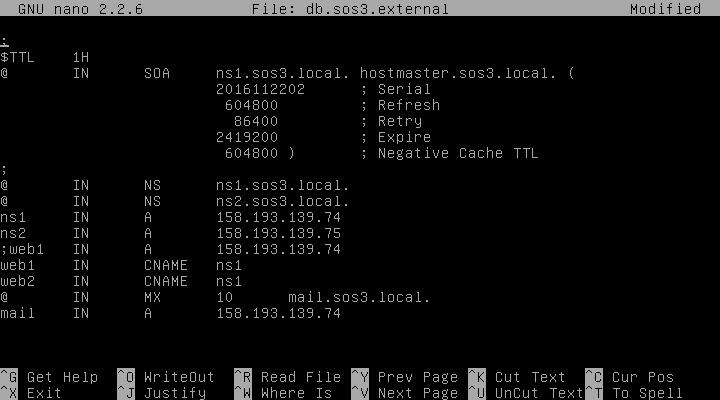
\includegraphics[scale=0.79]{linux_master_external}
\caption{Verejné DNS záznamy}
\label{fig:x dns_external}
\end{figure}

\begin{figure}[!htb]
\centering
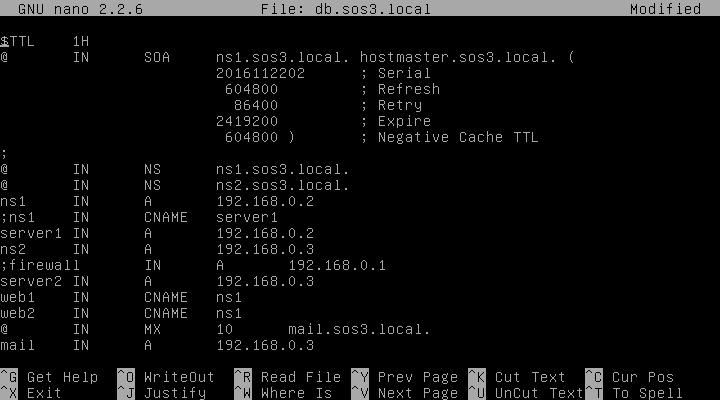
\includegraphics[scale=0.79]{linux_master_local}
\caption{Vnútorné DNS záznamy}
\label{fig:x dns_internal}
\end{figure}

\begin{figure}[!htb]
\centering
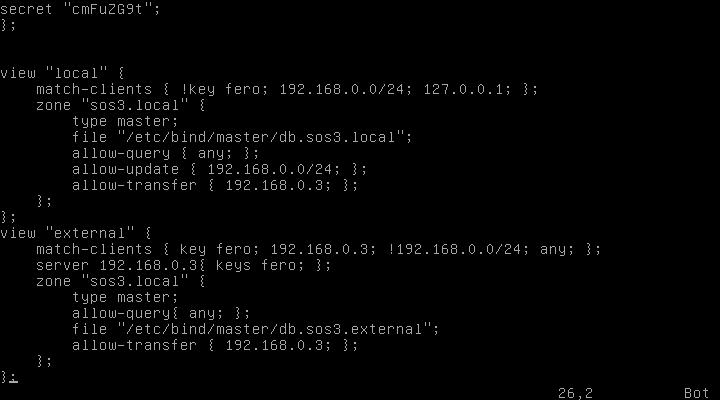
\includegraphics[scale=0.79]{linux_dns_views}
\caption{Konfigurácia DNS pohľadov}
\label{fig:x dns_views}
\end{figure}

\begin{figure}[!htb]
\centering
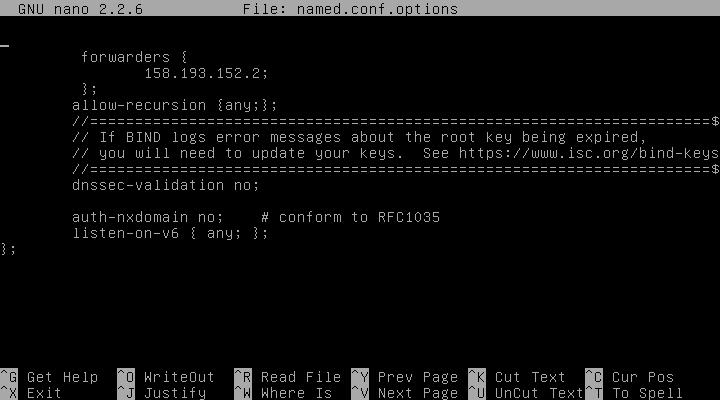
\includegraphics[scale=0.79]{linux_named_options}
\caption{Konfigurácia DNS forwardera}
\label{fig:x dns_forwarder}
\end{figure}


\section{DHCP}
\paragraph{}
DHCP server (S2) sme museli upraviť tak, aby prideľoval aj DNS adresy serverov. Súbor \say{/etc/dhcp/dhcpd.conf} na S1 sme upravili tak, že sme doň pridali privátne IP adresy DNS serverov (option domain-name-servers). Do časti pre podsieť sme definovali názvy týchto serverov. Voľbu \say{optionhost-name} sme zmenili z pôvodného \say{example.org} na \say{sos3.local}. Tým, že sme nastavili DNS server, nemusíme meniť na jednotlivých hostoch súbor \say{/etc/resolv.conf}.
\paragraph{}
Dynamic Host Configuration Protocol (DHCP) je súbor zásad, ktoré využívajú komunikačné zariadenia (počítač, router alebo sieťový adaptér), umožňujúci zariadeniu vyžiadať si a získať IP adresu od servera, ktorý má zoznam adries voľných na použitie.DHCP Server (Dynamic Host Configuration Protocol) vykonáva automatické pridelenie IP adries svojim klientom. Môžu to byť akékoľvek systémy, podporujúce DHCP. DHCP je štandardný protokol, môžu ho využívať aj systémy mimo Microsoft. Z Microsoft operačných systémov podporujú funkciu DHCP klienta všetky až na veľmi exotický LAN Manager pre OS / 2. V rámci siete potom máme DHCP Server - prideľujúca adresy a počítače - ktoré je od neho preberajú (DHCP Clients). V sieti môžu byť aj počítače, ktoré majú tieto adresy nastavené manuálne.

\begin{figure}[!htb]
\centering
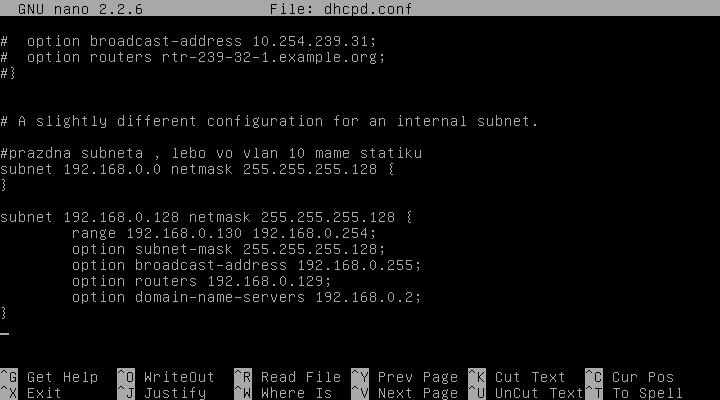
\includegraphics[scale=0.79]{linux_dhcp}
\caption{Konfiguračný súbor pre DHCP}
\label{fig:x dhcp_config}
\end{figure}

\section{NTP}
\paragraph{}
NTP(Network Time Protocol) je protokol na sychronizáciu všetkých počítačov pripojených do vnutornej siete. Tento protokol zaisťuje, aby všetky počítače v sietei mali rovnaký a presný čas. Bol nvrhnutý aby odolával následkom premenlivého zdržania pri doručovaní paketov. NTP používa UDP na porte 123. NTP server sme zvolili server2, ktorý má ip adresu 192.168.0.3. Nainštalovali sme NTP príkazom apt-get install ntp. Na klientoch sme nainštalovali NTP pomocou príkazu apt-get install ntp ntpdate. V súbore na serveri s2 /etc/ntp.conf sme pridali slovenské servery zo stránky www.pool.ntp.org/zone/sk. a ostatné servery sme zakomentovali. Klienti si z master serveru aktualizujú čas.

\begin{figure}[!htb]
\centering
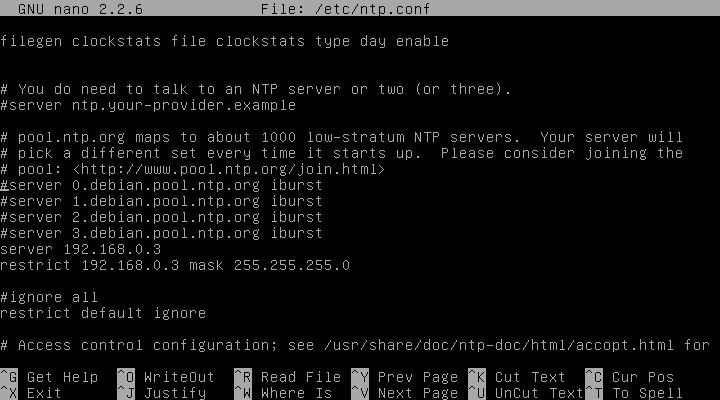
\includegraphics[scale=0.79]{linux_ntp_konfiguracia_server}
\caption{Konfigurácia NTP servera}
\label{fig:x ntp_config_server}
\end{figure}

\begin{figure}[!htb]
\centering
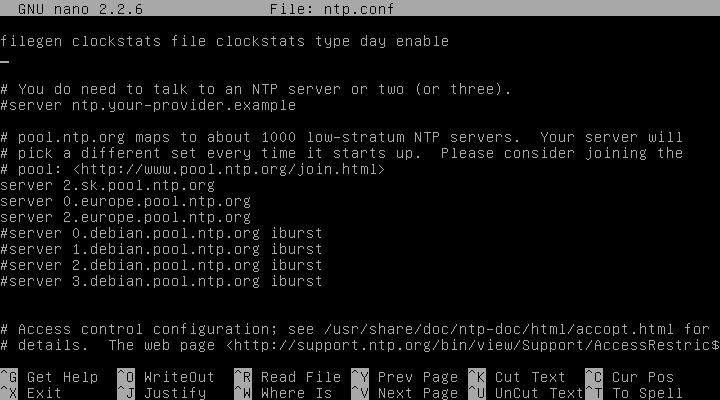
\includegraphics[scale=0.79]{linux_ntp_konfiguracia_klient}
\caption{Konfigurácia NTP na klientovi}
\label{fig:x ntp_config_client}
\end{figure}

\begin{figure}[!htb]
\centering
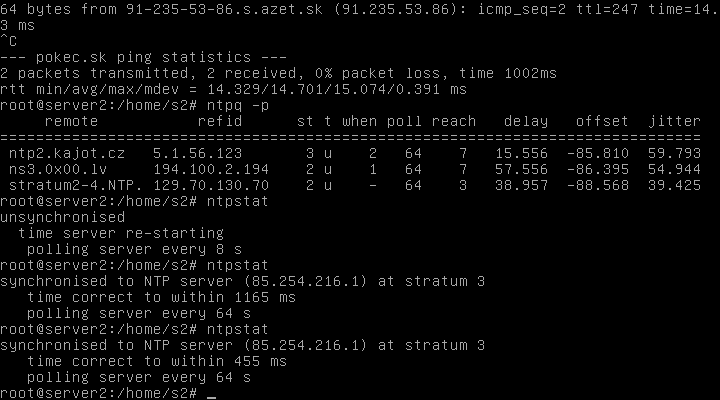
\includegraphics[scale=0.79]{linux_ntp_1}
\caption{Kontrola externých NTP serverov}
\label{fig:x ntp_config_valid_1}
\end{figure}

\begin{figure}[!htb]
\centering
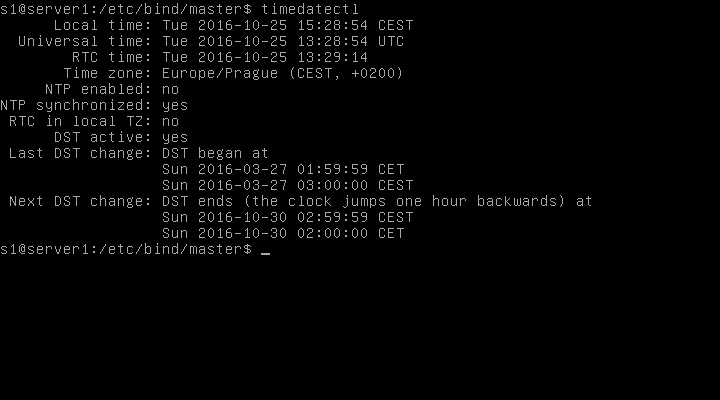
\includegraphics[scale=0.79]{linux_ntp_2}
\caption{Stav synchronizácie s NTP serverom}
\label{fig:x ntp_config_valid_2}
\end{figure}

\section{Web server}
\paragraph{}
Apache HTTP Server je softwarový webový server s Opensource licenciou pre Linux, BSD, Microsoft Windows a iné platformy.
\paragraph{}
PHP (PHP: Hypertext Preprocessor) je populárny opensource skriptovací jazyk, ktorý sa používa najmä na programovanie klient-server aplikácií (na strane servera) a pre vývoj dynamických webových stránok.
\paragraph{}
MySQL je slobodný a otvorený viacvláknový, viacužívateľský SQL relačný databázový server. MySQL je podporovaný na viacerých platformách (ako Linux, Windows či Solaris) a je implementovaný vo viacerých programovacích jazykoch ako PHP, C++ či Perl. Databázový systém je relačný, typu DBMS (database management system). Každá databáza je v MySQL tvorená z jednej alebo z viacerých tabuliek, ktoré majú riadky a stĺpce. V riadkoch sa rozoznávajú jednotlivé záznamy, stĺpce udávajú dátový typ jednotlivých záznamov, pracuje sa s nimi ako s poľami. Práca s MySQL databázou je vykonávaná pomocou takzvaných dotazov, ktoré vychádzajú z programovacieho jazyka SQL (StructuredQueryLanguage).
\paragraph{}
Na webový server sme použili apache. Apache HTTP Server je softwarový webový server s Opensource licenciou pre Linux, BSD, Microsoft Windows a iné platformy. V dnešnej dobe je najrozšírenejším na celom svete. Pre plnú fukncionalitu webového servera sme museli nainštalovať apache, mysql, php príkazom \say{apt-get install apache2 mysql php5} .
\paragraph{}
V adresári /var/www/ sme vytvorili priečinky s názvami web1 a web2. Kde web1 a web2 predstavovali dva virutálne webové servery. Následne sme v etc/apache2/sites-available 003-wiki.sos3.local.conf sme pridali cestu ku web stránke /var/www/web1 a ServerName web2.sos3.local. Pre joomlu v súbore 002-joomla.sos3.local.conf sme pridlai cestu k adresaru ked uz DocumentRoot /var/www/web1 a ServerName web1.sos3.local
\paragraph{}
Následne do DNS záznamov sme museli pridať:\\

\noindent
{\fontfamily{qcr}\selectfont

% Urob text mensi, aby sa vosiel na sirku obrazovky
\begin{small}

% Pouzijeme "verbatim", aby sme escapeovali cely odsek
\begin{verbatim}

db.sos1.local
web1 IN A 192.168.0.4
web2 IN A 192.168.0.4

db.sos1.public
web1 IN A 158.193.139.74
web2 IN A 158.193.139.74

\end{verbatim}

\end{small}

}

\subsection{Joomla}
\paragraph{}
V priečinku /var/www/web2 sme stiahli joomlu verziu 3.6 pomocou príkazu \say{wget https://github.com/.../Joomla\_3.6.0-Stable-Full\_Package.zip} . V ďalšom kroku sme odzipovali tento súbor príkazom \say{unzip Joomla\_3.6.0-Stable-Full\_Package.zip} . Následne sme v prehliadači otvorili web1.sos3.local a podľa príslušných krokov sme nainštalovali joomlu.

\subsection{Mediawiki}
\paragraph{}
V priečinku var/www/web1 sme stiahli Wikimedia pomocou príkazu \say{wget https://www.mediawiki.org/wiki/Download/mediawiki-1.2.8.zip} . Následne sme odzipovali tento súbor príkazom \say{unzip mediawiki-1.2.8.zip} . A v poslednom kroku sme v prehliadači web2.sos3.local nainštalovali mediawiki.

\begin{figure}[!htb]
\centering
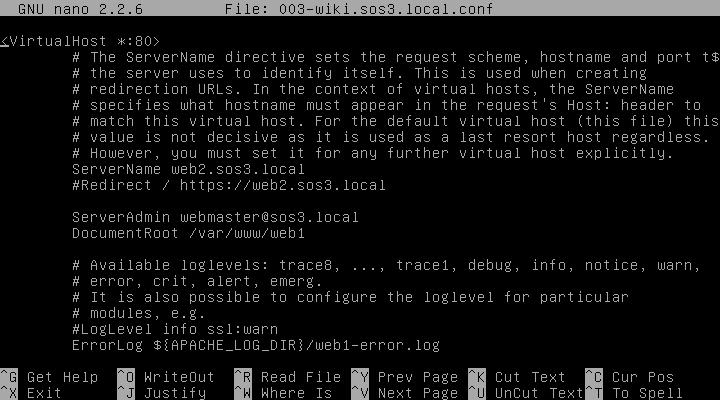
\includegraphics[scale=0.79]{linux_web1_konfiguracia}
\caption{Konfiguračný súbor webstránky}
\label{fig:x web1_config_file}
\end{figure}

\begin{figure}[!htb]
\centering
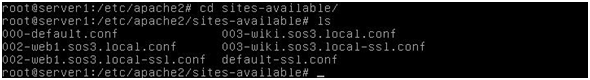
\includegraphics[scale=0.97]{linux_web_konfiguraky_webstranok}
\caption{Prehľad konfiguračných súborov webstránok}
\label{fig:x web_config_files_list}
\end{figure}

\section{Poštový server}
\paragraph{}
Na poštový server sme použili postfix.Postfix je počítačový program pre unixové systémy pro prepravu elektronickej pošty (MTA).
\paragraph{}
Najprv bolo ptorebné nainštalovať postfix príkazom apt-get installpostfix prešli sme inštaláciou kde sme nastavili hostname sos3.local. Následne sme museli reštartovať postfixservicepostfixrestart. V súbore /etc/postfix/main.cf je potrebné upraviť myhostname = sos3.local, odkomentovať\\
\paragraph{}
pridat konfigurak a obrazky

\section{Firewall}
\paragraph{}
Firewall sme konfigurovali priebežne s úlohami počas semestra. Nižšie je uvedený konfiguračný skript na pridávanie záznamov do \say{iptables}.

\noindent
{\fontfamily{qcr}\selectfont
\\

% Urob text mensi, aby sa vosiel na sirku obrazovky
\begin{small}

% Pouzijeme "verbatim", aby sme escapeovali cely odsek
\begin{verbatim}

#!/bin/bash

I=/sbin/iptables

#vycisti povodne pravidla
$I -F -t filter
$I -F -t nat

#zakaz vsetko, co nie je vyslovene povolene
#$I -P INPUT DROP
#$I -P FORWARD DROP
$I -P INPUT ACCEPT
$I -P FORWARD ACCEPT

#povol loopback
$I -A INPUT -i lo -j ACCEPT

########## STAVOVY FIREWALL ##########
#FW CONNTRACK - nastav sledovanie aktivnych pripojeni inicializovanych z FW
#Co odide z firewallu, sa vrati na firewall
$I -A INPUT -i eth0 -m conntrack --ctstate ESTABLISHED,RELATED -j ACCEPT

#VLAN CONNTRACK - aby sa nam vsetko z netu vratilo na VLANy
#Co odide z VLANiek, sa vrati do VLANiek
$I -A FORWARD -i eth0 -o eth1.10 -m conntrack --ctstate ESTABLISHED,RELATED -j ACCEPT
$I -A FORWARD -i eth0 -o eth1.20 -m conntrack --ctstate ESTABLISHED,RELATED -j ACCEPT

########## SNAT ##########
$I -t nat -A POSTROUTING -o eth0 -j SNAT --to-source 158.193.139.74
#a co s druhou ipckou? treba na nu tiez prekladat? mozme pridat aj nat na druhu ip

########## VLAN ROUTING ############
#Povol routing medzi vlanami
$I -A FORWARD -i eth1.10 -o eth1.20 -j ACCEPT
$I -A FORWARD -i eth1.20 -o eth1.10 -j ACCEPT

########## ICMP ############
#Povol pingy na fw
$I -A INPUT -p icmp -j ACCEPT

#Povol pingy z VLANiek von
$I -A FORWARD -i eth1.10 -o eth0 -p icmp -j ACCEPT
$I -A FORWARD -i eth1.20 -o eth0 -p icmp -j ACCEPT


########## SSH ##########
#Povol SSH na firewall zvonku aj zvnutra
$I -A INPUT -p tcp --dport 22 -j ACCEPT


########## SSH ##########
#Povol SSH na firewall zvonku aj zvnutra
$I -A INPUT -p tcp --dport 22 -j ACCEPT

#Navrat SSH na FW
$I -A INPUT -i eth1.10 -p tcp --sport 22 -j ACCEPT
$I -A INPUT -i eth1.20 -p tcp --sport 22 -j ACCEPT

#Povol spatne SSH z vnutornej siete na FW
$I -A INPUT -i eth1.10 -p tcp --sport 22 -j ACCEPT
$I -A INPUT -i eth1.20 -p tcp --sport 22 -j ACCEPT

#S1 SSH zvonku dnu
$I -t nat -A PREROUTING -d 158.193.139.74 -p tcp --dport 3002 -j DNAT 
	--to-destination 192.168.0.2:22
$I -A FORWARD -p tcp -d 192.168.0.2 --dport 22 -j ACCEPT
$I -A FORWARD -p tcp -s 192.168.0.2 --sport 22 -j ACCEPT

#S2 SSH zvonku dnu
$I -t nat -A PREROUTING -d 158.193.139.74 -p tcp --dport 3003 -j DNAT 
	--to-destination 192.168.0.3:22
$I -A FORWARD -p tcp -d 192.168.0.3 --dport 22 -j ACCEPT
$I -A FORWARD -p tcp -s 192.168.0.3 --sport 22 -j ACCEPT

#S1 zvnutra von
$I -A FORWARD -d 192.168.0.2 -p tcp --dport 22 -j ACCEPT
$I -A FORWARD -s 192.168.0.2 -p tcp --sport 22 -j ACCEPT

#S2 zvnutra von
$I -A FORWARD -d 192.168.0.3 -p tcp --dport 22 -j ACCEPT
$I -A FORWARD -s 192.168.0.3 -p tcp --sport 22 -j ACCEPT

########## DNS ############
#Povol DNS na FW
$I -A INPUT -p udp --sport 53 -j ACCEPT
$I -A INPUT -p udp --dport 53 -j ACCEPT

#Povol DNS zvnutra von
$I -A FORWARD -i eth1.10 -o eth0 -p tcp --dport 53 -j ACCEPT
$I -A FORWARD -i eth1.10 -o eth0 -p udp --dport 53 -j ACCEPT
$I -A FORWARD -i eth1.20 -o eth0 -p tcp --dport 53 -j ACCEPT
$I -A FORWARD -i eth1.20 -o eth0 -p udp --dport 53 -j ACCEPT

#MASTER DNS (S1) lokalne
$I -A FORWARD -d 192.168.0.2 -p tcp --dport 53 -j ACCEPT
$I -A FORWARD -s 192.168.0.2 -p tcp --sport 53 -j ACCEPT
$I -A FORWARD -d 192.168.0.2 -p udp --dport 53 -j ACCEPT
$I -A FORWARD -s 192.168.0.2 -p udp --sport 53 -j ACCEPT
#SLAVE DNS (S2) lokalne
$I -A FORWARD -d 192.168.0.3 -p tcp --dport 53 -j ACCEPT
$I -A FORWARD -s 192.168.0.3 -p tcp --sport 53 -j ACCEPT
$I -A FORWARD -d 192.168.0.3 -p udp --dport 53 -j ACCEPT

#S1 DNS zvonku dnu
$I -t nat -A PREROUTING -d 158.193.139.74 -p tcp --dport 53 -j DNAT 
	--to-destination 192.168.0.2
$I -t nat -A PREROUTING -d 158.193.139.74 -p udp --dport 53 -j DNAT 
	--to-destination 192.168.0.2

#S2 DNS zvonku dnu
$I -t nat -A PREROUTING -d 158.193.139.75 -p tcp --dport 53 -j DNAT 
	--to-destination 192.168.0.3
$I -t nat -A PREROUTING -d 158.193.139.75 -p udp --dport 53 -j DNAT 
	--to-destination 192.168.0.3

#Povovl DNS zvoknu dnu
$I -A FORWARD -i eth0 -o eth1.10 -d 192.168.0.2 -p udp --dport 53 -j ACCEPT
$I -A FORWARD -i eth0 -o eth1.10 -d 192.168.0.3 -p udp --dport 53 -j ACCEPT

########## NTP ##########
#Povol NTP na FW
$I -A INPUT -p udp --sport 123 -j ACCEPT

#Povol pripojenia na NTP server
$I -A FORWARD -d 192.168.0.3 -i eth1.10 -p udp --sport 123 -j ACCEPT

#Povol NTP vnutri
$I -A FORWARD -d 192.168.0.3 -p udp --dport 123 -j ACCEPT
$I -A FORWARD -s 192.168.0.3 -p udp --sport 123 -j ACCEPT

#NTP DNAT - Povol NTP zvonku dnu
$I -t nat -A PREROUTING -d 158.193.139.74 -p udp --dport 123 -j DNAT 
	--to-destination 192.168.0.3:123
$I -t nat -A PREROUTING -d 158.193.139.75 -p udp --dport 123 -j DNAT 
	--to-destination 192.168.0.3:123

########## HTTP ##########
#Povol HTTP von
$I -A FORWARD -i eth1.10 -o eth0 -p tcp --dport 80 -j ACCEPT
$I -A FORWARD -i eth1.20 -o eth0 -p tcp --dport 80 -j ACCEPT

#HTTP lokalne
$I -A FORWARD -d 192.168.0.2 -p tcp --dport 80 -j ACCEPT
$I -A FORWARD -s 192.168.0.2 -p tcp --sport 80 -j ACCEPT

#HTTP zvonku dnu
$I -t nat -A PREROUTING -d 158.193.139.74 -p tcp --dport 80 -j DNAT 
	--to-destination 192.168.0.2

########## HTTPS ##########
#Povol HTTPS von
$I -A FORWARD -i eth1.10 -o eth0 -p tcp --dport 443 -j ACCEPT
$I -A FORWARD -i eth1.20 -o eth0 -p tcp --dport 443 -j ACCEPT

#HTTPS lokalne
$I -A FORWARD -d 192.168.0.2 -p tcp --dport 443 -j ACCEPT
$I -A FORWARD -s 192.168.0.2 -p tcp --sport 443 -j ACCEPT

#HTTP zvonku dnu
$I -t nat -A PREROUTING -d 158.193.139.74 -p tcp --dport 443 -j DNAT 
	--to-destination 192.168.0.2

########## FTP ##########
#Povol FTP von
$I -A FORWARD -i eth1.10 -o eth0 -p tcp --dport 20 -j ACCEPT
$I -A FORWARD -i eth1.10 -o eth0 -p tcp --dport 21 -j ACCEPT
$I -A FORWARD -i eth1.20 -o eth0 -p tcp --dport 20 -j ACCEPT
$I -A FORWARD -i eth1.20 -o eth0 -p tcp --dport 21 -j ACCEPT

########## DHCP ##########
#Povol DHCP
#$I -I FORWARD -i eth1.10 -p udp --dport 67:68 --sport 67:68 -j ACCEPT
#$I -I FORWARD -i eth1.20 -p udp --dport 67:68 --sport 67:68 -j ACCEPT

########## SMTP ##########
$I -t nat -A PREROUTING -p tcp --dport 25 -j DNAT --to-destination 192.168.0.3:25
$I -A FORWARD -p tcp -d 192.168.0.3 --dport 25 -j ACCEPT
$I -A FORWARD -p tcp -s 192.168.0.3 --sport 25 -j ACCEPT

########## IMAP ##########
$I -A FORWARD -p tcp -d 192.168.0.3 --dport 143 -j ACCEPT
$I -A FORWARD -p tcp -s 192.168.0.3 --sport 143 -j ACCEPT

# Pridaj logovanie do /var/messages/kern.log kvoli debuggingu
$I -A INPUT -j LOG
$I -A FORWARD -j LOG

# Zapni Forwarding pre iptables (aby fungovali "FORWARD" prikazy)
echo 1 > /proc/sys/net/ipv4/ip_forward

\end{verbatim}

\end{small}

}

\subsection{Spúšťanie iptables skriptu po štarte}
\paragraph{}
Skript na pridávanie záznamov \say{iptables} spúšťame príkazom \say{up} vrámci konfigurácií sieťového rozhrania \say{eth0} v súbore \say{/etc/network/interfaces}, ktorý je uvedený nižšie.

\noindent
{\fontfamily{qcr}\selectfont

% Urob text mensi, aby sa vosiel na sirku obrazovky
\begin{small}

% Pouzijeme "verbatim", aby sme escapeovali cely odsek
\begin{verbatim}

source /etc/network/interfaces.d/*

# The loopback network interface
auto lo
iface lo inet loopback
# The primary network interface
allow-hotplug eth0
iface eth0 inet static
        address 158.193.139.74
        netmask 255.255.255.0
        gateway 158.193.139.1
up /usr/local/etc/firewall.sh

auto eth0:1
allow-hotplug eth0:1
iface eth0:1 inet static
        address 158.193.139.75
        netmask 255.255.255.0
        gateway 158.193.139.1

# Vnutorna (firemna) sietovka
auto eth1

#VLAN 10 subinterface
auto eth1.10
iface eth1.10 inet static
        address 192.168.0.1
        netmask 255.255.255.128
        dns-nameservers 192.168.0.2 192.168.0.3

#VLAN 20 subinterface
auto eth1.20
iface eth1.20 inet static
        address 192.168.0.129
        netmask 255.255.255.128
        dns-nameservers 192.168.0.2 192.168.0.3

# This is an autoconfigured IPv6 interface
iface eth0 inet6 auto

\end{verbatim}

\end{small}

}

\chapter{Windows}
\section{DHCP}
\paragraph{}
Inštaláciu sme vykonali vo Windows service manager - Add Roles and Features, vybrali si možnosť DHCP server.
\paragraph{}
Pre konfiguráciu sme klikli na TOOLS a následne DHCP.Zobrazilo sa nám okno s ponukou , my sme vybrali náš server, IPv4 a možnosť new scope. Spustil sa New ScopeWizard. V prvom kroku  sme napisali názov pravidla na prideľovanie IP adries. Ďalej sme zvolili  rozsah IP adries a masku.
\\
\\
Rozsah IP adries od 192.168.0.1 po 192.168.0.254\\
Maska 255.255.255.0
\paragraph{}
Následne sme využili možnosti pridať výnimku z predtým zadaného rozsahu, teda adresy ktoré sa nebudu prideľovať napriek tomu, že sú zo nami  zadaného rozsahu v predchádzajúcom kroku. Ide o adresy serverov 192.168.0.2 a 192.168.0.3.
\paragraph{}
Potom  sme zvolili aký dlhý čas si server bude pamätať IP adresy ktoré niekomu pridelil. Stačilo nám 5 hodín (dĺžka cvičenia aj s rezervou).
\paragraph{}
Nakoniec sme nastavili bránu na „192.168.1.1”, pridali sme IP adresy našich DNS serverov, teda  „192.168.1.2“ a „192.168.1.3”. , a dokončili inštaláciu kliknutím na Finish.

\section{DNS}
\paragraph{}
V prvom rade sme si zvolili Master a Slave. Master je server1 (192.168.0.2) a Slave server2 (192.168.0.1)
\paragraph{}
DNS master nainštalujeme pomocou Windows Server Manager. Klikneme na Manage , vyberieme možnosť Add roles and features daľej Role-based or feature-basedinstallation, zobrazí sa  zoznam serverov, my vyberieme náš server a zvolímezo zoznamu rolesDNS Server a dokončíme inštaláciu.
\paragraph{}
Po inštalácií DNS balíka sme sa dostali cez Tools -\textgreater{} DNS -\textgreater{} Configure a DNS server -\textgreater{} Create a forward lookupzone k vytvoreniuprimárnej forward lookupzóny sos1.local , nastavili sme aj  nech záznamy preposiela na Slave 192.168.0.3.
\paragraph{}
Prešli sme k inštalácii DNS Slave.Postup ako pri DNS Master avšak  DNS server bolo potrebné nastaviť na slavemode. Vybrali sme  Tools -\textgreater{} Forward lookupzones -\textgreater{} New zone. Hneď v prvom kroku sme vybrali  možnosť nie Primaryzone ale Secondaryzone a taktiež  meno zóny .V ďalšom kroku určíme DNS Masterserver,v našom riešení ma  IP 192.168.0.2 .Dokončíme vytváranie zóny pomocou Next a Finish. Onedlho si Slave stiahne záznamy z DNS Master servera.

\section{NTP}
\paragraph{}
Na spustenie NTP na Windows servery sme museli vykonať zmeny v registroch. Spustíme okno RUN  (WIN+R) , kde napíšeme regedit. Následne sa dostaneme cestou HKEY\_LOCAL\_MACHINE | SYSTEM | CurrentControlSet | Services | W32Time | TimeProviders | NtpServer	až k hodnote Enabled , ktorá bola nastavená na 0 , a my ju zmeníme na 1.Využijeme opäť win+R , zadáme w32tm /config /update,čím vlastne spustíme NTP server na danom zariadení.
\paragraph{}
Na aplikáciu  zmien sme reštartovali Windows Timeservice príkazom zadaným do commandline:
\\
\\
net stop w32time \&\& net start w32tim.

\section{NAT}
\paragraph{}
Nainštalovanie sme vykonali vo Windows Server Manageri, kde cez Add Roles and Features. Pridali sme
\\
\\
imidž
\paragraph{}
potvrdili sme službu Routing a následne sme ju nainštalovali. Pri inštalácii zvolíme sie\v{t}ový adaptér eth0, ktorý je pripojený k internetu. Po inštalácii je NAT plne funkčné, ale je potrebné prida\v{t} NAT záznamy na porte 53.  Ďalej sme ho potrebovali nakonfigurovať v control panel -\textgreater{} Administrative tools -\textgreater{} Routing and Remote Access. Po kliknutí na NAT, vyberieme záložku s adaptérom, ktorý je pripojený k internet. V Address Pool je potrebné nastavi\v{t} from, čo znamená našu počiatočnú public adresu 158.193.139.74 a to, čo je naša koncová adresa 158.193.139.75 a maska 255.255.255.0. V záložke services and ports je potrebné prida\v{t} 4 nové záznamy NAT pre DNS(Master-Slave, TCP-UDP).

\section{Web server}
\paragraph{}
Webserver ISS (Internet Information Server) sme pridali cez windows server manager tlačidlom Addroles and features, kde sme vyhľadali Web Server ISS a pokračujeme ďalej. Pri ponuke Role Services
\paragraph{}
Následne nainštalujeme služby na server. Po úspešnej inštalácii sa IIS objaví na \v{l}avom paneli v server manager-i. Klikneme na ikonu IIS a v zozname dostupných serverov sa zjaví jeden - ten, na ktorom uskuto\v{c}\v{n}ujeme konfiguráciu. Klikneme na\v{n} pravým tla\v{c}idlom myši a z ponuky zvolíme možnos\v{t} Internet Information Services (IIS) Manager. Otvorí sa nové okno, v ktorého \v{l}avom paneli sa nachádza náš server. Rozbalíme jeho ponuku a klikneme na Sites. Pravý klik na Default Web Site nám ponúkne viacero možností vrátane nastavenia webstránky a pridania novej.

\paragraph{}
Po inštalácii sa nachádza ISS v ľavom paneli vo Windows Server Manager-i. Po kliknutí na tools v pravom hornom rohu klikneme Internet Information Services (ISS) manager. A po rozkliknutí na ľavom rohu je už vytvorená default sites. Otvoriť ju je možné zadaním do browseru “localhost”.

\section{Poštový server}
\paragraph{}
V server manageri klikneme na tools a v záložne DNS, nasmerujume sa ku DNS severu a vytvoríme nové záznamy pre mail server. Cname záznam mail 158.193.139.74, dva MX(Mail exchanger) záznamy 0 mail sos3.local a 10 mail sos3.local.
\paragraph{}
Zo stránky mailenable.com stiahneme standart edition. Začneme inštaláciou stiahnutého balíčka, zaklikneme web mail service(server). V nasledujúcich krokoch napíšeme do Domain Name: sos3.local a DNS host: 192.168.0.2 a smtp port: 25. Počas inštalácie nám vybehne tabuľká, kde odklikneme aby sa mailserver inštaloval ako webserver ISS. V server manageri po kliknutí servers -> localhost -> system -> diagnose si skontrolujeme či všetky políčka sú pass, čo nám značí že mail enable funguje. V ďalšom kroku servers -> localhost -> services and connectors  a na SMTP klikneme pravým tlačidlom a klikneme na properties. V záložne general nastavíme default mail domain name čo je v našom prípade mail.sos3.local. Ďalej v záložke smart host nastavíme IP/DOMAIN 158.193.139.74. Po reštarte serveru vidíme že, všetky service sú running.


\chapter{Záver}
Lorem ipsum dolor sit amet, consectetur adipisicing elit, sed do eiusmod tempor incididunt ut labore et dolore magna aliqua. Ut enim ad minim veniam, quis nostrud exercitation ullamco laboris nisi ut aliquip ex ea commodo consequat. Duis aute irure dolor in reprehenderit in voluptate velit esse cillum dolore eu fugiat nulla pariatur. Excepteur sint occaecat cupidatat non proident, sunt in culpa qui officia deserunt mollit anim id est laborum.

Lorem ipsum dolor sit amet, consectetur adipisicing elit, sed do eiusmod tempor incididunt ut labore et dolore magna aliqua. Ut enim ad minim veniam, quis nostrud exercitation ullamco laboris nisi ut aliquip ex ea commodo consequat. Duis aute irure dolor in reprehenderit in voluptate velit esse cillum dolore eu fugiat nulla pariatur. Excepteur sint occaecat cupidatat non proident, sunt in culpa qui officia deserunt mollit anim id est laborum \parencite[see][p10]{latexcompanion}.

Lorem ipsum dolor sit amet, consectetur adipisicing elit, sed do eiusmod tempor incididunt ut labore et dolore magna aliqua. Ut enim ad minim veniam, quis nostrud exercitation ullamco laboris nisi ut aliquip ex ea commodo consequat. Duis aute irure dolor in reprehenderit in voluptate velit esse cillum dolore eu fugiat nulla pariatur. Excepteur sint occaecat cupidatat non proident, sunt in culpa qui officia deserunt mollit anim id est laborum \parencite[compare][]{knuthwebsite}.

Lorem ipsum dolor sit amet, consectetur adipisicing elit, sed do eiusmod tempor incididunt ut labore et dolore magna aliqua. Ut enim ad minim veniam, quis nostrud exercitation ullamco laboris nisi ut aliquip ex ea commodo consequat. Duis aute irure dolor in reprehenderit in voluptate velit esse cillum dolore eu fugiat nulla pariatur. Excepteur sint occaecat cupidatat non proident, sunt in culpa qui officia deserunt mollit anim id est laborum \parencite[e.g.][page 300]{einstein}.


\printbibliography

\end{document}
